\documentclass[aspectratio=1610]{beamer}

\usetheme{unnslides}
\usefonttheme{professionalfonts}

\usepackage[T2A]{fontenc}
\usepackage[utf8]{inputenc}
\usepackage{listings}
\usepackage{graphicx}
\usepackage{caption}
\usepackage{cmbright}
\usepackage{fontspec}
\usepackage{amsfonts}
\usepackage{subfig}
\usepackage{tikz}

\captionsetup[subfigure]{labelformat=empty}
\captionsetup[figure]{labelformat=empty}

\setmainfont{Latin Modern Sans}
\setromanfont{Latin Modern Sans}
\setsansfont{Latin Modern Sans}

\setlength{\tabcolsep}{1pt}

%\setbeamertemplate{itemize item}{\color{black}$\blacktriangleright$}

\DeclareMathOperator*{\argmax}{arg\,max}
\DeclareMathOperator*{\argmin}{arg\,min}
\DeclareMathOperator{\sign}{sign}
\DeclareMathOperator{\re}{Re}

\graphicspath{ {../poster/images/}{img/} }

%set pages numeration
\newcommand\numbered{\setbeamertemplate{footline}{%
  \vspace{-10em}
   \raisebox{5pt}{\makebox[\paperwidth]{%
     \hfill\makebox[10pt]{%
       \usebeamerfont{footline}\usebeamercolor[fg]{footline}
       \insertframenumber}}}}}
\newcommand\unnumbered{\setbeamertemplate{footline}{}}

\title{Towards Efficient and Data Agnostic Image Classification Training Pipeline for Embedded Systems}
\author{\textbf{Kirill~Prokofiev}$^{1,}$$^2$ \and \textbf{Vladislav~Sovrasov}$^{1,}$$^3$}
\institute{$^1$Intel , $^2$Higher School of Economics, $^3$Nizhny Novgorod State University}
\date{}

\begin{document}
\numbered
{
\unnumbered
\begin{frame}[noframenumbering,plain]
\titlepage
\end{frame}
}

\begin{frame}
  \frametitle{Image classification task}
  Points:
    \begin{itemize}
      \item Extended classification task statement. VTAB benchmark.
      \item Datasets and validation protocol.
      \item Efficient model architectures.
      \item Training pipeline.
      \item Results. Comparison with other approaches.
    \end{itemize}
\end{frame}


\begin{frame}
  \frametitle{Datasets}
  \begin{table}
    \caption{Image classification datasets which were used for training.}
    \label{tab:data}
    \centering
    \begin{tabular}{l|c|c|c}
      Dataset & Number of classes & \multicolumn{2}{c}{Number of Images} \\
              &                   & Train     &   Validation \\ \hline
      Oxford-IIIT Pets & 37 & 3680 & 3369 \\
      Describable Textures (DTD)$^*$ & 47 & 4826 & 814 \\
      Oxford 102 Flowers$^*$ & 102 & 6614 & 1575 \\
      Caltech 101$^*$ & 101 & 6941 & 1736 \\
      Cars Dataset & 196 & 8144 & 8041 \\
      Birdsnap$^*$ & 500 & 47386 & 2443 \\
      CIFAR-100 & 100 & 50000 & 10000 \\
      Fashion-MNIST & 10 & 60000 & 10000 \\
      SVHN & 10 & 73257 & 26032 \\
      Food-101 & 101 & 75750 & 25250 \\
      SUN397$^*$  & 397 & 92440 & 16314 \\
      \hline
      \multicolumn{4}{l}{\footnotesize{$^*$ for experiments on these datasets we do custom random splits.}}
    \end{tabular}
  \end{table}
\end{frame}

\begin{frame}
  \frametitle{Evaluation protocol. Metrics}
  Like in VTAB, we use averaged across datasets accuracy metrics:
  \begin{itemize}
      \item Average top-1 accuracy.
      \item Average mean average precision:
      \begin{displaymath}
        mAP=\frac{\sum_{q=1}^Q AP(q)}{Q}=\frac{\sum_{i=1}^N AP(i)}{N}=\frac{1}{N}\sum_{i=1}^N \frac{1}{K_i},
      \end{displaymath}
    \end{itemize}
    \(mAP\) metrics allows revealing ranking ability of a classification algorithm by accumulating all rank-k metrics.

\end{frame}

\begin{frame}
  \frametitle{Mutual learning. Loss functions}
  \begin{displaymath}
    \label{eq:equationDML}
    \begin{split}
      L_{fast}(x) = L_{CE}(p_1(x), y) + D_{KL}(p_2(x) || p_1(x))\\
      L_{slow}(x) = L_{AMS}(p_2(x), y) + D_{KL}(p_1(x) || p_2(x))
    \end{split}
  \end{displaymath}
  \begin{figure}
    \subfloat[]
      {{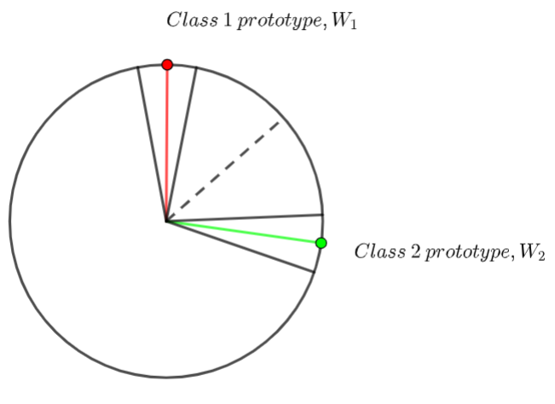
\includegraphics[width=.3\textwidth]{amsm.png} }}
  \end{figure}
\end{frame}

{
\unnumbered
\begin{frame}{{}}
  \frametitle{Q\&A}
  \begin{center}
    kirill.prokofiev@intel.com@intel.com

    vladislav.sovrasov@intel.com

    \url{https://github.com/openvinotoolkit/training_extensions/}
  \end{center}
\end{frame}
}
\end{document}
